\chapter{Inverse Solutions}
\label{ch:inv}

\section{Overview}

The inverse problem of electrocardiography is to find suitable electrical source parameters on the heart that adequately describe the observed body surface potentials. Regularization is typically employed in solution methods to reduce the sensitivity of the problem to relatively small errors in the observed body surface potentials, thereby stabilizing it. As a result, solution methods may be supplied body surface potentials, a forward model, and method-specific regularization parameters as input. Specific use of each method is described below. As output, modules primarily produce the resulting solution with extra outputs, depending on the specific method.

\section{Descriptions of the Inverse Solution Methods Implemented in SCIRun}

%%%%%%%%%%%%%%%%%%%%%%%
\subsection{Tikhonov Regularization}\label{sec:inverse:tikhonov}
    
    As described in Sec.~\ref{sec:math_tikhonov}, Tikhonov regularization is a classical inverse method that solves the following least squares problem:
    \begin{center}
        \begin{eqnarray}
            min_{X} \| P (Y - A X) \|^{2}_{2} + \lambda^{2} \| RX \|^{2}_{2},
        \label{eq:inverseSec_tik_problem}
        \end{eqnarray}
    \end{center}
    where $Y$ are the measured ECG potentials, $A$ is the forward matrix, $X$ are the unknown potentials on the heart, $\lambda$ is the regularization parameter, $R$ is a regularization matrix and $P$ is the sensor covariance matrix. 
    All these variables can be found as inputs or outputs of the module \href{http://scirundocwiki.sci.utah.edu/SCIRunDocs/index.php/CIBC:Documentation:SCIRun:Reference:BioPSE:SolveInverseProblemWithTikhonov}{{\tt SolveInverseProblemWithTikhonov}}, shown in \autoref{fig:tik_module}.
    \begin{figure}
        \begin{center}
        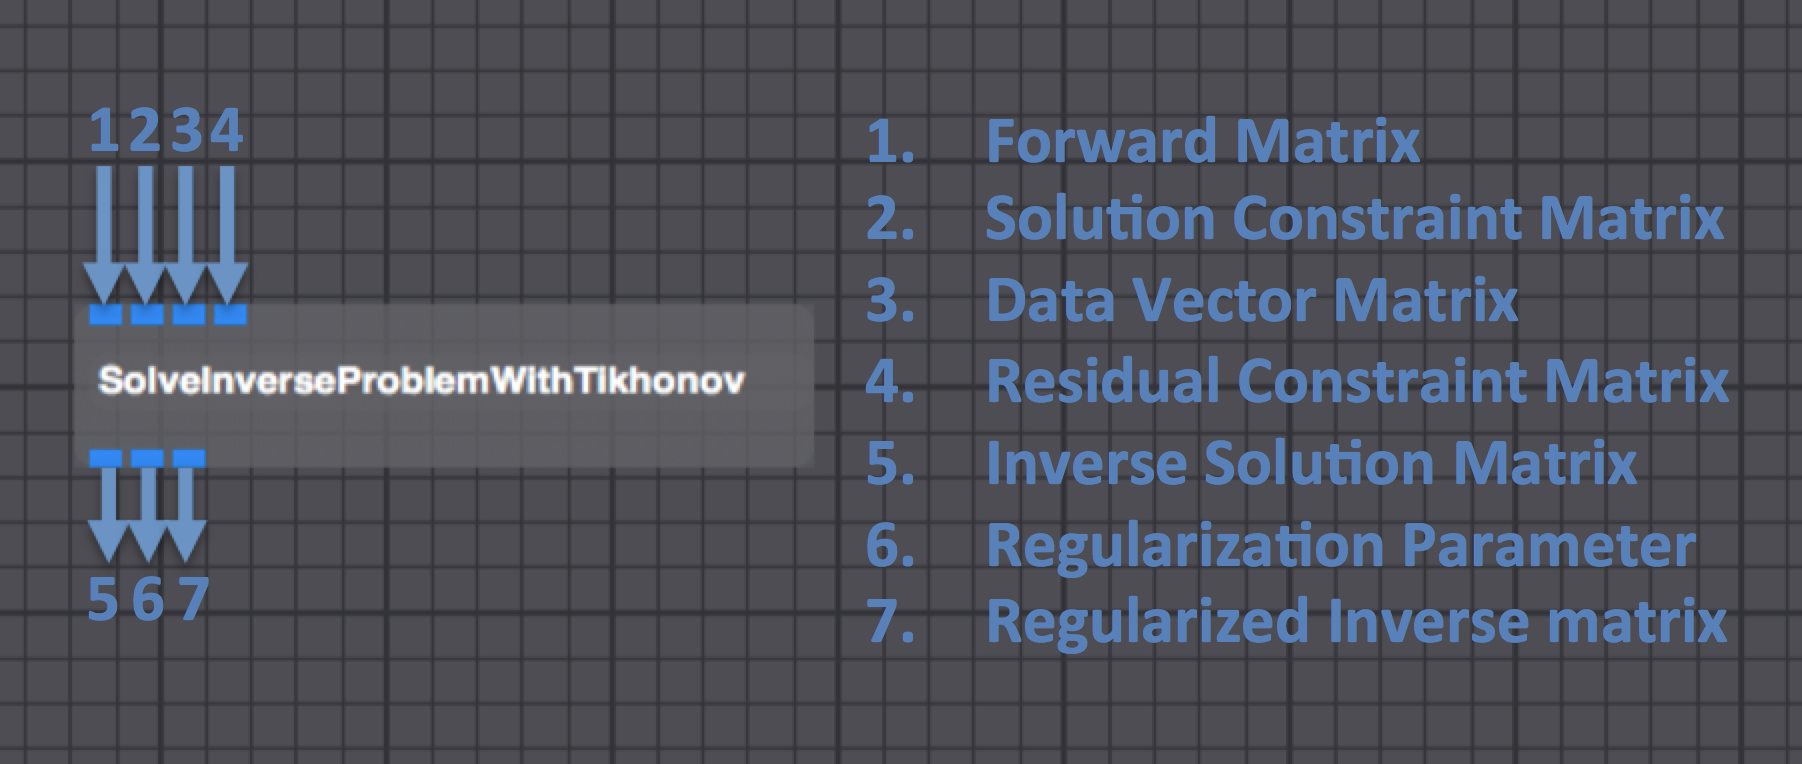
\includegraphics[width=0.7\textwidth]{ECGToolkitGuide_figures/tik1.png}
        \caption{Revised Tikhonov module: {\tt SolveInverseProblemWithTikhonov}.  }
        \label{fig:tik_module}
        \end{center}
    \end{figure}
    \noindent{\bf Inputs:}
    \begin{enumerate}
        \item Forward Matrix ($A\in\Re^{N,M}$)
        \item Weights in Source Space ($R\in\Re^{L,M}$ or squared $R^2\in\Re^{M,M}$ o)
        \item Measured Potentials ($Y\in\Re^{N,T}$)
        \item Weights in Sensor Space ($P\in\Re^{F,N}$ or squared $P^2\in\Re^{N,N}$),
    \end{enumerate}
    {\bf Outputs:}
     \begin{enumerate}
        \item Inverse Solution ($X\in\Re^{M,T}$)
        \item Regularization Parameter ($\lambda$)
        \item Regularized Inverse ($G\in\Re^{M,N}$)
    \end{enumerate}

    An example of the usage of the module \href{http://scirundocwiki.sci.utah.edu/SCIRunDocs/index.php/CIBC:Documentation:SCIRun:Reference:BioPSE:SolveInverseProblemWithTikhonov}{{\tt SolveInverseProblemWithTikhonov}} can be found in the network ``potential-based-inverse/tikhonov-inverse.srn5'', which is shown in \autoref{TikhonovNetworkExample}.
    This example network is composed of four main blocks:
    \begin{itemize}
        \item {\bf Loading Data (green):} These are the modules that load the data into SCIRun.
        \item {\bf Forward Solution (white):} These modules compute simulations of ECG potentials that would be measured on the body surface.
        \item {\bf Tikhonov Inverse (black):} This module computes the Tikhonov inverse solution.
        \item {\bf Visualization (purple):} These modules provide visualization of the solution and the ground truth.
    \end{itemize}
    
    \subsubsection{Options and Modes of Operation}
    
    The \href{http://scirundocwiki.sci.utah.edu/SCIRunDocs/index.php/CIBC:Documentation:SCIRun:Reference:BioPSE:SolveInverseProblemWithTikhonov}{{\tt SolveInverseProblemWithTikhonov}} module allows for multiple modes of operation that provide different functionalities and computational advantages.
    These modes of operation, can be found in the two panels of the module user interface, shown in \autoref{fig:tik_module_gui}. 
    The options within each of the two panels are described in the following:
    
    \begin{figure}
    \begin{center}
    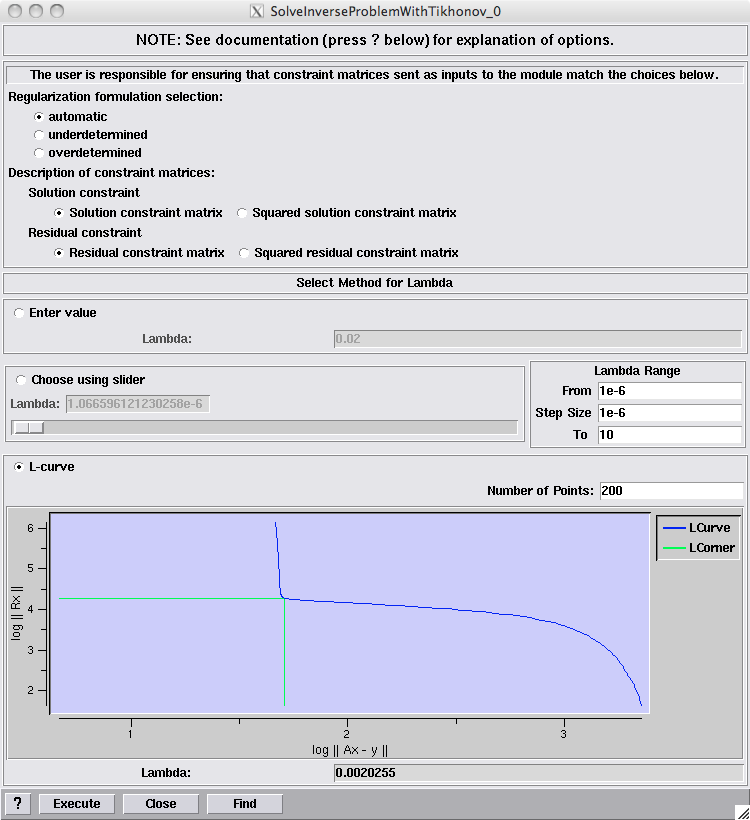
\includegraphics[width=0.45\textwidth]{ECGToolkitGuide_figures/tik2.png}
    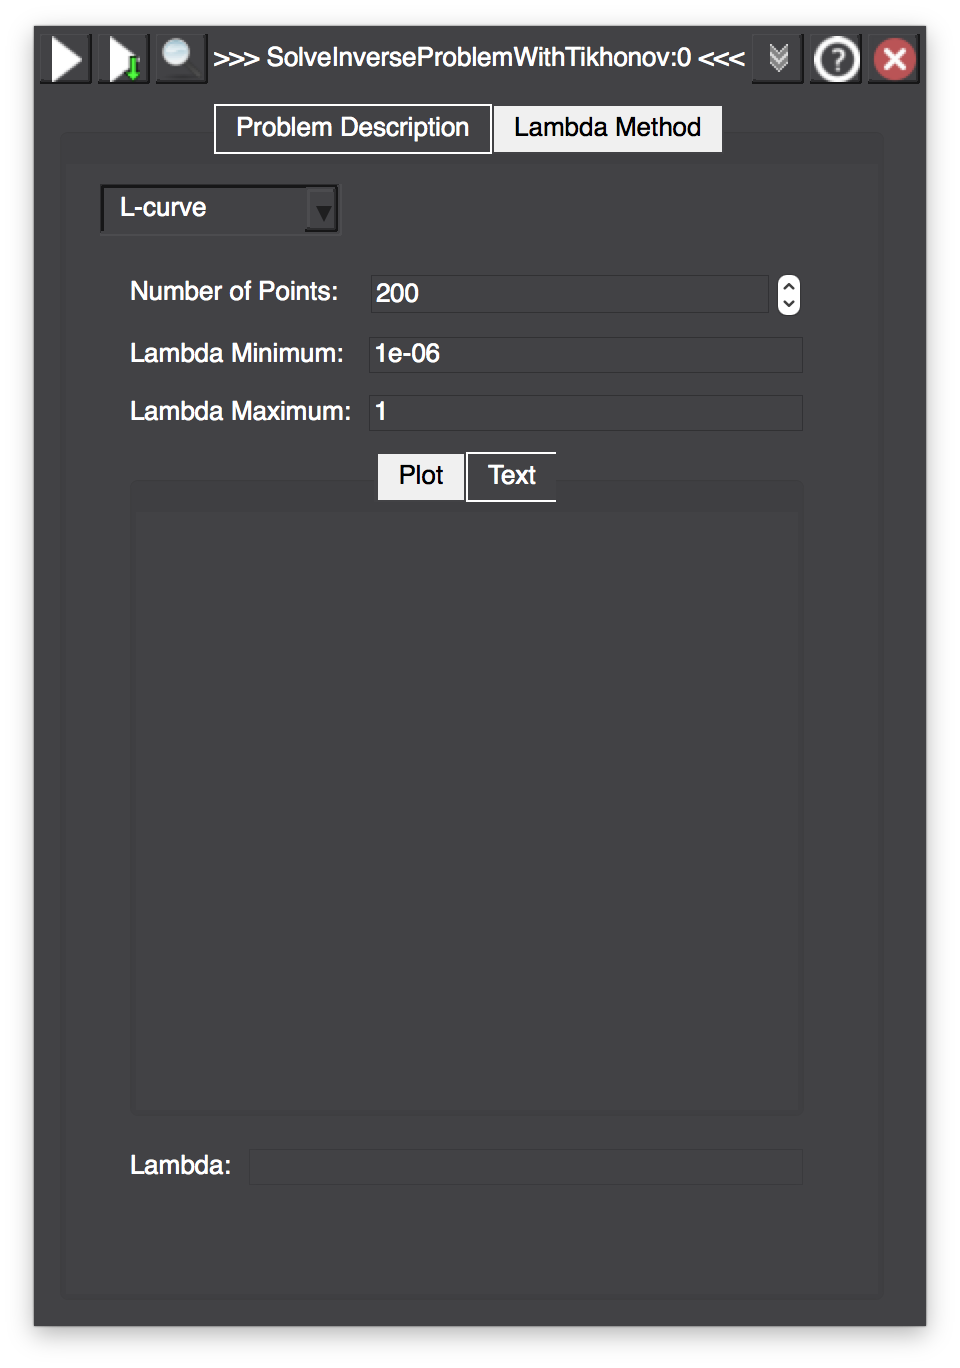
\includegraphics[width=0.45\textwidth]{ECGToolkitGuide_figures/tik3.png}
    \caption{GUI from revised Tikhonov module. Left: problem description. Right: Lambda selection method {\tt SolveInverseProblemWithTikhonov}.}
    \label{fig:tik_module_gui}
    \end{center}
    \end{figure}

    \noindent{\bf Problem Description:}
    
    There are two formulations for the solutions of least squares problem in \autoref{eq:inverseSec_tik_problem}.
    These are the overdetermined formulation:
    \begin{center}
    \begin{eqnarray}
        \hat{x}   &=& \left(A^T P^TPA + \lambda^{2}R^TR\right)^{-1} A^T P^TP Y,
    \label{eq:inverseSec_TikhonovSolutions1}
    \end{eqnarray}
    \end{center}    
    and the underdetermined:
    \begin{center}
    \begin{eqnarray}
        \hat{x}  &=& (R^TR)^{-1} A^T \left( A(R^TR)^{-1}A^T + \lambda^2 (P^TP)^{-1}  \right)^{-1}Y.
    \label{eq:inverseSec_TikhonovSolutions2}
    \end{eqnarray}
    \end{center}
    The difference between these two formulations is computational. 
    It can be observed from equations \ref{eq:inverseSec_TikhonovSolutions1} and \ref{eq:inverseSec_TikhonovSolutions2} that the size of the inverse matrix that needs to be computed is $N$ in the overdetermined case and $M$ in the underdetermined.
    Thus, when the number of ECG measurements is smaller than the number of sources on the heart ($N<M$), it is computationally desirable to use \autoref{eq:inverseSec_TikhonovSolutions1}.
    On the other hand, if the number of ECG measurements is larger than the number of sources ($N>M$), it is preferable to use \autoref{eq:inverseSec_TikhonovSolutions2}.
    \href{http://scirundocwiki.sci.utah.edu/SCIRunDocs/index.php/CIBC:Documentation:SCIRun:Reference:BioPSE:SolveInverseProblemWithTikhonov}{{\tt SolveInverseProblemWithTikhonov}} is prepared to use either formulation upon request of the user or choose it automatically based on the size of the forward matrix.
    To choose the desired option, the user must select the appropriate radial button in the ``Regularization Formulation'' option within the  ``Problem Description'' panel.
    
    The ``Problem Description'' panel also allows to modify how the source and sensor weight matrices ($R$ and $P$) are defined.
    As can be observed in equations \ref{eq:inverseSec_TikhonovSolutions1} and \ref{eq:inverseSec_TikhonovSolutions2}, these two matrices appear in quadratic form. For this reason, many users might prefer to define them in the quadratic form (i.e. $R^2=R^TR$ and $C^2=C^TC$).
    \href{http://scirundocwiki.sci.utah.edu/SCIRunDocs/index.php/CIBC:Documentation:SCIRun:Reference:BioPSE:SolveInverseProblemWithTikhonov}{{\tt SolveInverseProblemWithTikhonov}} allows users to change the default definition of these input matrices to the squared form by selecting the appropriate radial buttons in the ``Constraint Matrices'' options within the  ``Problem Description'' panel.
    
    
    \noindent{\bf Lambda Method:}
    
    The solutions to the Tikhonov regularization problem depend on the selection of the regularization parameter ($\lambda$).
    There are multiple approaches in the literature that allow for its selection.
    \href{http://scirundocwiki.sci.utah.edu/SCIRunDocs/index.php/CIBC:Documentation:SCIRun:Reference:BioPSE:SolveInverseProblemWithTikhonov}{{\tt SolveInverseProblemWithTikhonov}} is currently implemented so that the user can choose between a direct entry, selection using a slider and the L-curve method, described in Sec.~\ref{sec:math_regparam}.
    These methods can be found by selecting the appropriate option in the drop-down menu within the ``Lambda Method'' panel.
    
    
    \begin{figure}
        \begin{center}
        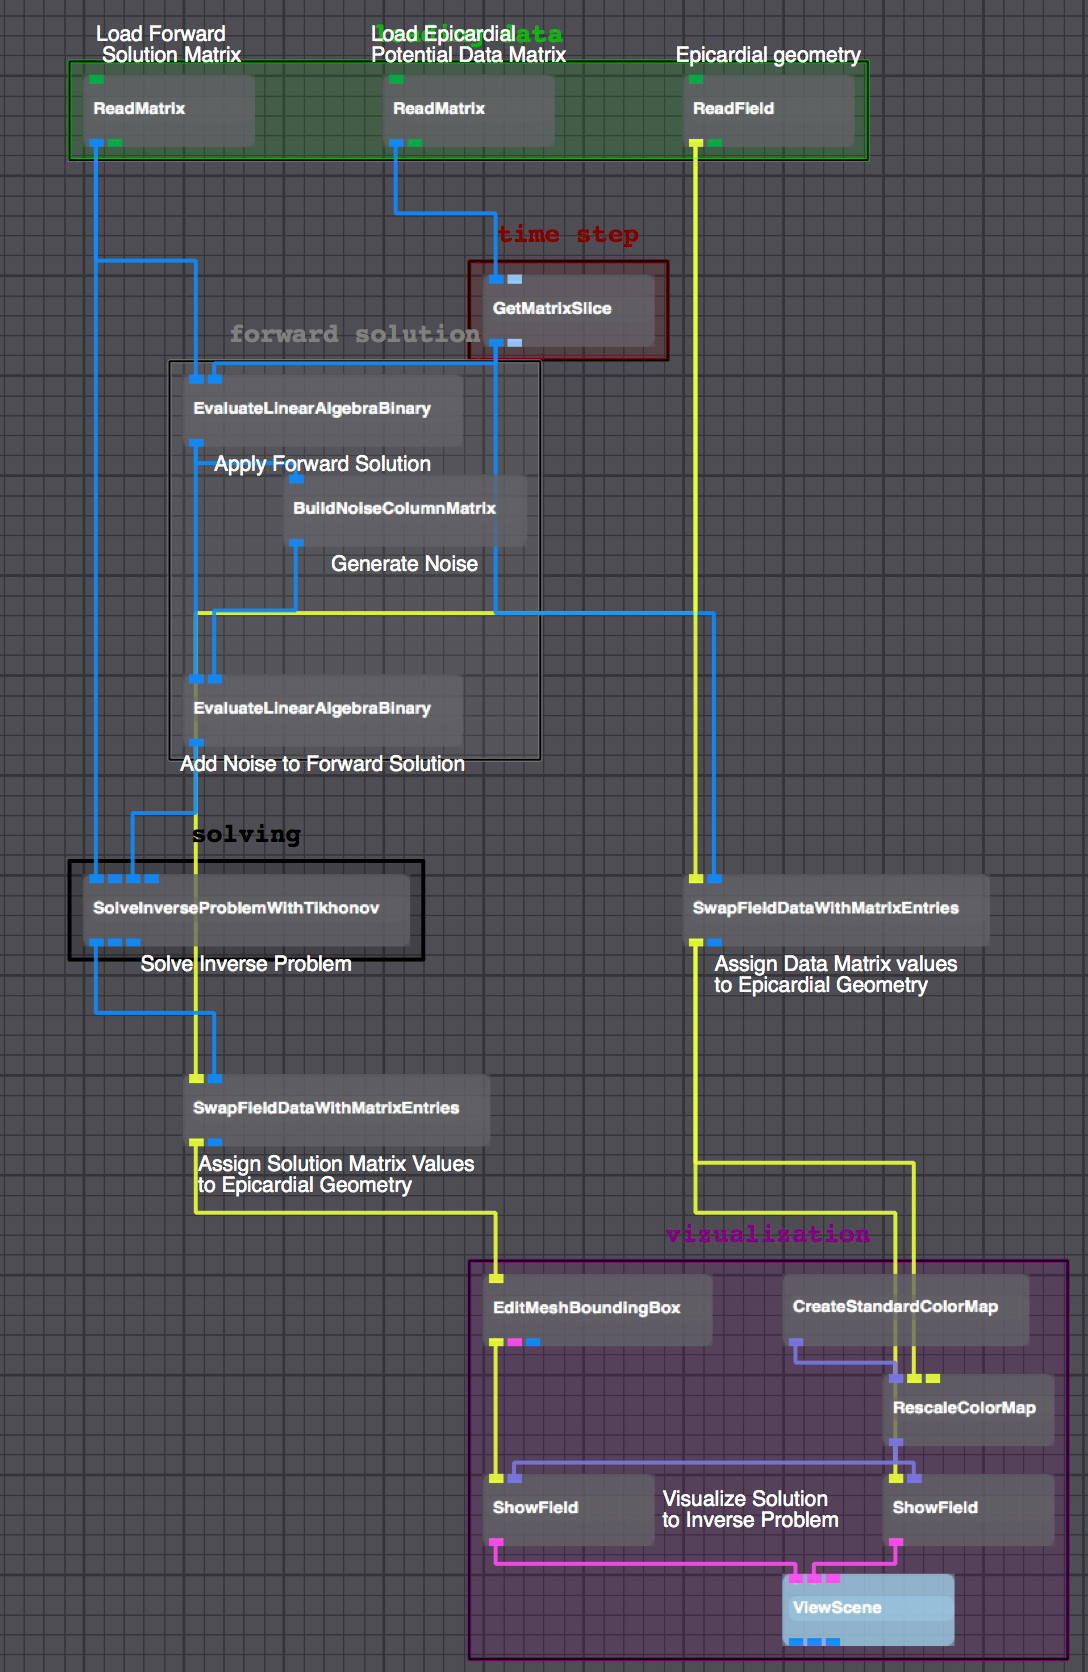
\includegraphics[width=0.9\textwidth]{ECGToolkitGuide_figures/TikhonovNetwork.png}
        \caption{The SCIRun network for the Tikhonov inverse solution example.}
        \label{TikhonovNetworkExample}
        \end{center}
    \end{figure}
    


    
\subsection{Tikhonov SVD Method}

    The Tikhonov SVD method effectively solves the same least squares problem as the Tikhonov method described above.
    The difference between these two implementations is computational. 
    The \href{http://scirundocwiki.sci.utah.edu/SCIRunDocs/index.php5/CIBC:Documentation:SCIRun:Reference:BioPSE:SolveInverseProblemWithTikhonovSVD}{{\tt SolveInverseProblemWithTikhonovSVD}} module uses the following formulation to solve the least-squares problem:
    \begin{center}
    \begin{eqnarray}
        \hat{X}   &=& \sum_{k=1}^K \frac{\sigma_k}{\lambda^2 + \sigma_k^2} v_k u_k^T Y,
    \label{eq:inverseSec_TikhonovSolutions1}
    \end{eqnarray}
    \end{center} 
    where $Y$ are the ECG measurements, $X$ are the unknown potentials on the heart, $\lambda$ is the regularization parameter and $\sigma_k$, $u_k$ and $v_k$ are the singular values, left and right singular vectors of the forward matrix $A$ and $K$ is its rank.
    
    The \href{http://scirundocwiki.sci.utah.edu/SCIRunDocs/index.php5/CIBC:Documentation:SCIRun:Reference:BioPSE:SolveInverseProblemWithTikhonovSVD}{{\tt SolveInverseProblemWithTikhonovSVD}} module is shown in \autoref{fig:tik_moduleSVD}.
    \begin{figure}
        \begin{center}
        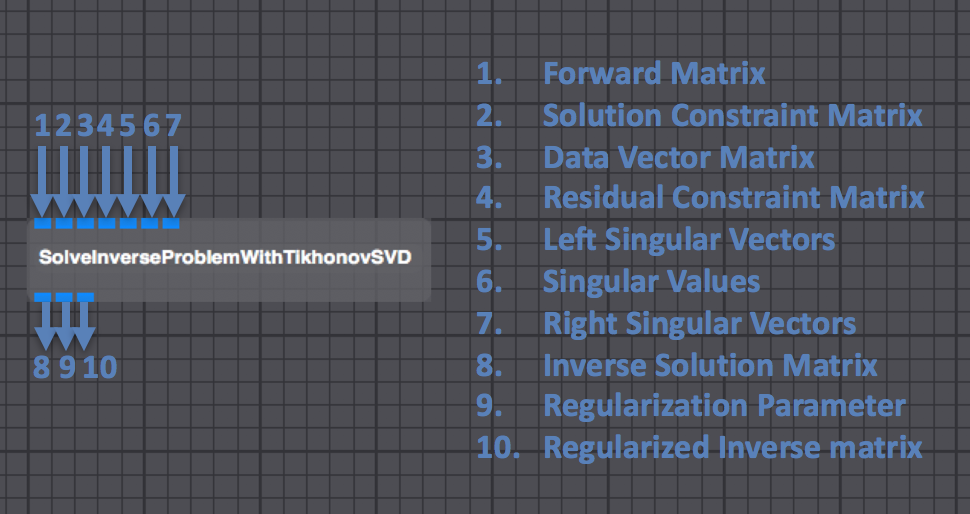
\includegraphics[width=0.7\textwidth]{ECGToolkitGuide_figures/TikhonovSVD_module.png}
        \caption{Revised TikhonovSVD module: {\tt SolveInverseProblemWithTikhonovSVD}.  }
        \label{fig:tik_moduleSVD}
        \end{center}
    \end{figure}
    The inputs and outputs of this module are a superset of \href{http://scirundocwiki.sci.utah.edu/SCIRunDocs/index.php/CIBC:Documentation:SCIRun:Reference:BioPSE:SolveInverseProblemWithTikhonov}{{\tt SolveInverseProblemWithTikhonov}}.
    The new additions permit the user to use pre-computed singular values and vectors of the forward matrix.
    \noindent{\bf Inputs:}
    \begin{enumerate}
        \item Forward Matrix ($A\in\Re^{N,M}$)
        \item Weights in Source Space ($R\in\Re^{L,M}$ or squared $R^2\in\Re^{M,M}$ o)
        \item Measured Potentials ($Y\in\Re^{N,T}$)
        \item Weights in Sensor Space ($P\in\Re^{F,N}$ or squared $P^2\in\Re^{N,N}$)
        \item Left Singular Vectors ($U\in\Re^{N,N}$ )
        \item Singular Values ($S\in\Re^{K,K}$ or in vector form $s\in\Re^{K,1}$)
        \item Right Singular Vectors ($V\in\Re^{M,M}$),
    \end{enumerate}
    {\bf Outputs:}
     \begin{enumerate}
        \item Inverse Solution ($X\in\Re^{M,T}$)
        \item Regularization Parameter ($\lambda$)
        \item Regularized Inverse ($G\in\Re^{M,N}$)
    \end{enumerate}
    
    \subsubsection{Options and Modes of Operation}
    
    The options allowed in \href{http://scirundocwiki.sci.utah.edu/SCIRunDocs/index.php5/CIBC:Documentation:SCIRun:Reference:BioPSE:SolveInverseProblemWithTikhonovSVD}{{\tt SolveInverseProblemWithTikhonovSVD}} include the use of a pre-computed singular value decomposition of the forward matrix and the method to select the regularization parameter $\lambda$.
    
    \noindent{\bf Pre-computed Singular Value Decompositions}
    
    When needed, \href{http://scirundocwiki.sci.utah.edu/SCIRunDocs/index.php5/CIBC:Documentation:SCIRun:Reference:BioPSE:SolveInverseProblemWithTikhonovSVD}{{\tt SolveInverseProblemWithTikhonovSVD}} automatically computes a Singular Value Decomposition of the input forward matrix using sub-routines found in the Eigen library.
    However, the module is also prepared to use a pre-computed singular value decomposition. 
    This option is selected by connecting ALL the input ports of the left and right singular vectors and singular values (ports 5, 6 and 7).
    In this case, the algorithm skips the computation of the SVD and uses the provided matrices.
    
    \noindent{\bf Lambda Method}
    
    The solutions to the TikhonovSVD regularization problem depend on the selection of the regularization parameter ($\lambda$).
    There are multiple approaches in the literature that allow for its selection.
    \href{http://scirundocwiki.sci.utah.edu/SCIRunDocs/index.php5/CIBC:Documentation:SCIRun:Reference:BioPSE:SolveInverseProblemWithTikhonovSVD}{{\tt SolveInverseProblemWithTikhonovSVD}} is currently implemented so that the user can choose between a direct entry, selection using a slider and the L-curve method, described in Sec.~\ref{sec:math_regparam}.
    These methods can be found by selecting the appropriate option in the drop-down menu within the ``Lambda Method'' panel as done in \href{http://scirundocwiki.sci.utah.edu/SCIRunDocs/index.php/CIBC:Documentation:SCIRun:Reference:BioPSE:SolveInverseProblemWithTikhonov}{{\tt SolveInverseProblemWithTikhonov}} (see \autoref{fig:tik_module_gui}).
    
    
    \begin{figure}
        \begin{center}
        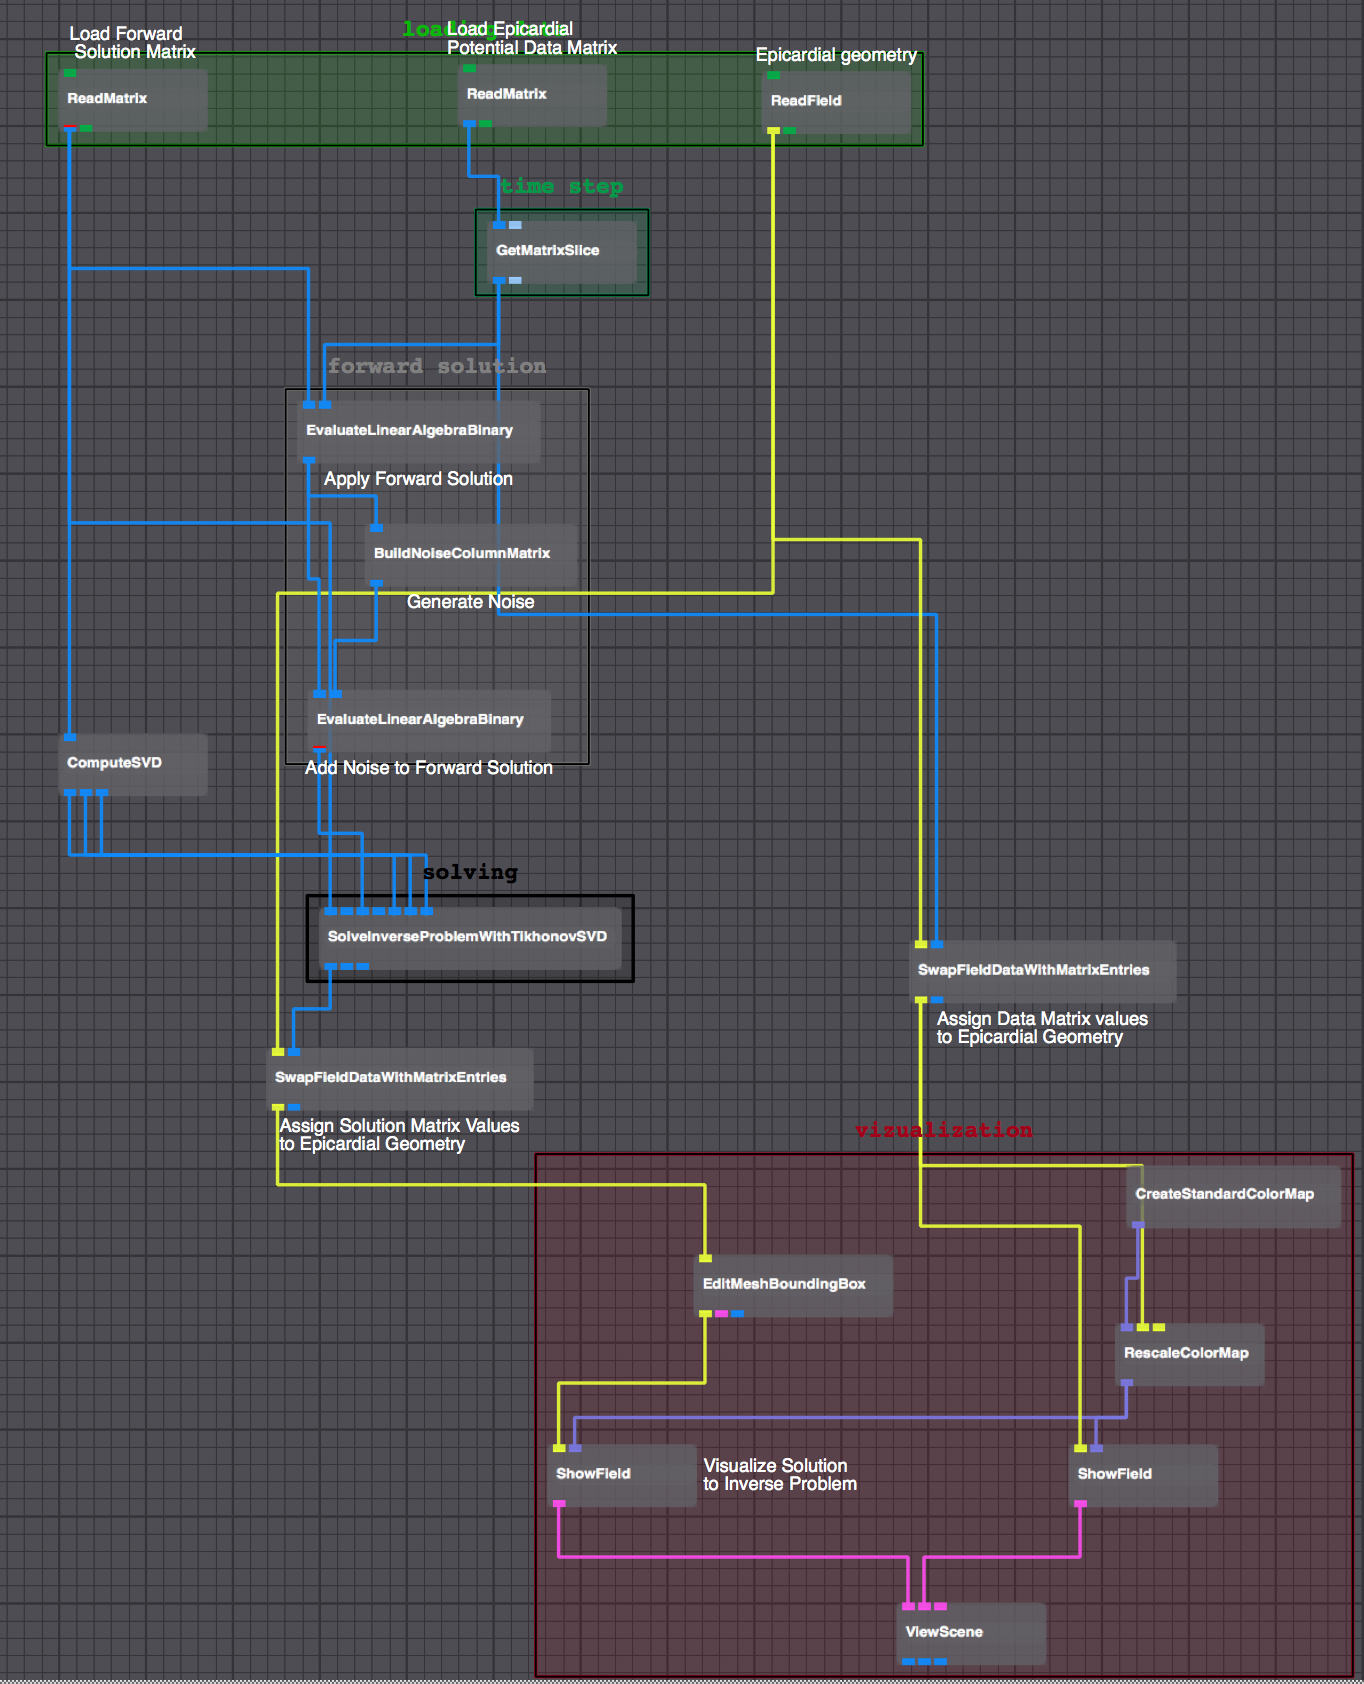
\includegraphics[width=0.9\textwidth]{ECGToolkitGuide_figures/TikhonovSVDNetwork.png}
        \caption{The SCIRun network for the TikhonovSVD inverse solution example.}
        \label{fig:TikhonovNetworkExampleSVD}
        \end{center}
    \end{figure}


  
\subsection{Truncated SVD Method (TSVD)}
    
    The truncated SVD method solves the classical least-squares problem with a low-rank approximation of the forward matrix. 
    Solutions to this method require the decomposition of the forward matrix $A$ into its left singular vectors $U$, the right singular vetors $V$ and the corresponding singular values $S$. 
    Then, these are computed following the formula:
    \begin{center}
    \begin{eqnarray}
        \hat{X}   &=& \sum_{k=1}^Q \frac{1}{\sigma_k} v_k u_k^T Y,
    \label{eq:inverseSec_TikhonovSolutions1}
    \end{eqnarray}
    \end{center} 
    where $Y$ are the ECG measurements, $X$ are the unknown potentials on the heart, $\lambda$ is the regularization parameter and $\sigma_k$, $u_k$ and $v_k$ are the singular values, left and right singular vectors of the forward matrix $A$ and $Q$ is the truncation point.
    
    The module \href{http://scirundocwiki.sci.utah.edu/SCIRunDocs/index.php5/CIBC:Documentation:SCIRun:Reference:BioPSE:SolveInverseProblemWithTSVD}{{\tt SolveInverseProblemWithTSVD}} is shown along its inputs and outputs in \autoref{fig:TSVD_module}
    \begin{figure}
        \begin{center}
        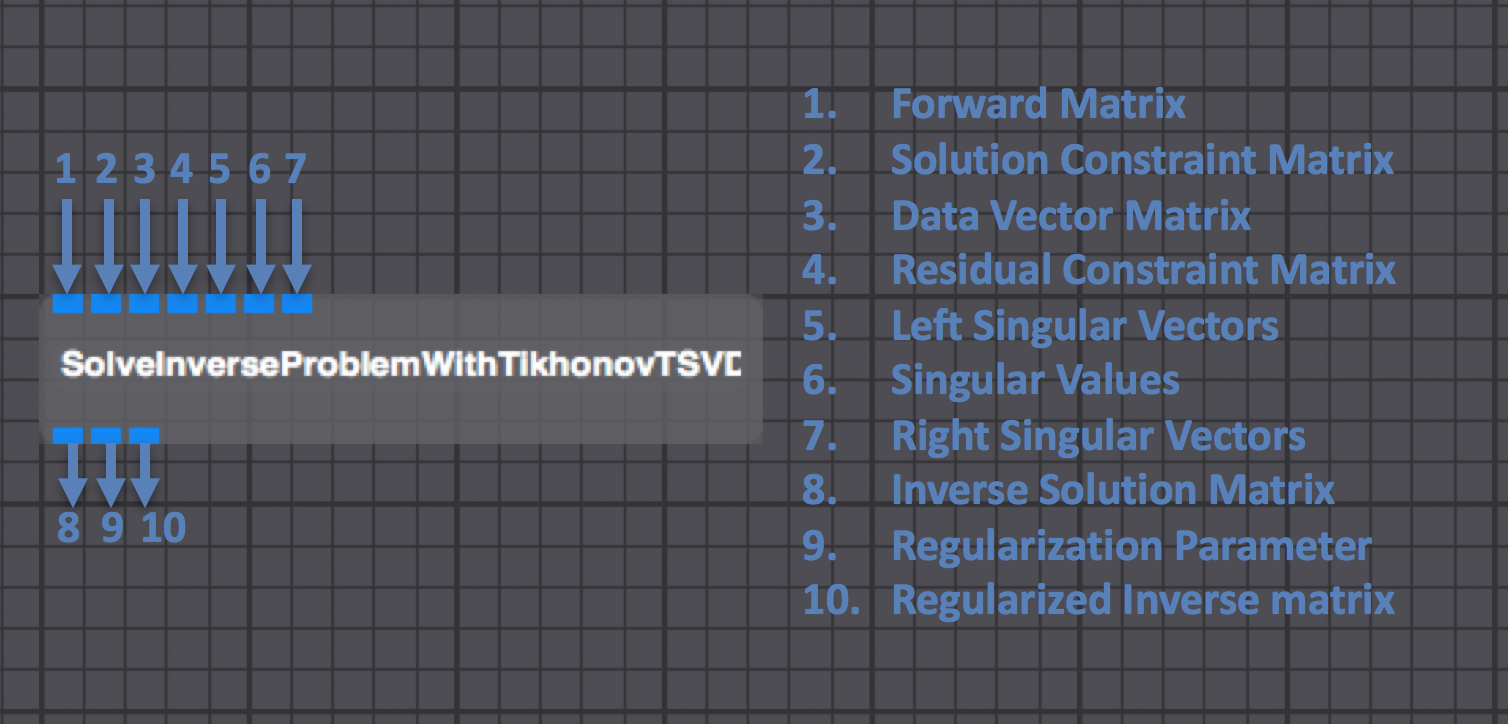
\includegraphics[width=0.7\textwidth]{ECGToolkitGuide_figures/TSVD_module.png}
        \caption{Revised TSVD module: {\tt SolveInverseProblemWithTSVD}.  }
        \label{fig:tik_moduleSVD}
        \end{center}
    \end{figure}
    The inputs and outputs of this module are a superset of \href{http://scirundocwiki.sci.utah.edu/SCIRunDocs/index.php/CIBC:Documentation:SCIRun:Reference:BioPSE:SolveInverseProblemWithTikhonov}{{\tt SolveInverseProblemWithTikhonov}}.
    The new additions permit the user to use pre-computed singular values and vectors of the forward matrix.
    \noindent{\bf Inputs:}
    \begin{enumerate}
        \item Forward Matrix ($A\in\Re^{N,M}$)
        \item Weights in Source Space ($R\in\Re^{L,M}$ or squared $R^2\in\Re^{M,M}$ o)
        \item Measured Potentials ($Y\in\Re^{N,T}$)
        \item Weights in Sensor Space ($P\in\Re^{F,N}$ or squared $P^2\in\Re^{N,N}$)
        \item Left Singular Vectors ($U\in\Re^{N,N}$ )
        \item Singular Values ($S\in\Re^{K,K}$ or in vector form $s\in\Re^{K,1}$)
        \item Right Singular Vectors ($V\in\Re^{M,M}$),
    \end{enumerate}
    {\bf Outputs:}
     \begin{enumerate}
        \item Inverse Solution ($X\in\Re^{M,T}$)
        \item Regularization Parameter ($\lambda$)
        \item Regularized Inverse ($G\in\Re^{M,N}$)
    \end{enumerate}
    
    
    \subsubsection{Options and Modes of Operation}
    
    The options allowed in \href{http://scirundocwiki.sci.utah.edu/SCIRunDocs/index.php5/CIBC:Documentation:SCIRun:Reference:BioPSE:SolveInverseProblemWithTikhonovSVD}{{\tt SolveInverseProblemWithTikhonovSVD}} include the use of a pre-computed singular value decomposition of the forward matrix and the method to select the truncation point (or regularization parameter) $Q$.
    
    \noindent{\bf Pre-computed Singular Value Decompositions}
    
    When needed, \href{http://scirundocwiki.sci.utah.edu/SCIRunDocs/index.php5/CIBC:Documentation:SCIRun:Reference:BioPSE:SolveInverseProblemWithTSVD}{{\tt SolveInverseProblemWithTSVD}} automatically computes a Singular Value Decomposition of the input forward matrix using sub-routines found in the Eigen library.
    However, the module is also prepared to use a pre-computed singular value decomposition. 
    This option is selected by connecting ALL the input ports of the left and right singular vectors and singular values (ports 5, 6 and 7).
    In this case, the algorithm skips the computation of the SVD and uses the provided matrices.
    
    \noindent{\bf Lambda Method}
    
    The solutions to the TSVD regularization problem depend on the selection of the regularization parameter ($Q$).
    There are multiple approaches in the literature that allow for its selection.
    \href{http://scirundocwiki.sci.utah.edu/SCIRunDocs/index.php5/CIBC:Documentation:SCIRun:Reference:BioPSE:SolveInverseProblemWithTSVD}{{\tt SolveInverseProblemWithTSVD}} is currently implemented so that the user can choose between a direct entry, selection using a slider and the L-curve method, described in Sec.~\ref{sec:math_regparam}.
    These methods can be found by selecting the appropriate option in the drop-down menu within the ``Lambda Method'' panel as done in \href{http://scirundocwiki.sci.utah.edu/SCIRunDocs/index.php/CIBC:Documentation:SCIRun:Reference:BioPSE:SolveInverseProblemWithTikhonov}{{\tt SolveInverseProblemWithTikhonov}} (see \autoref{fig:tik_module_gui}).


    \begin{figure}
        \begin{center}
        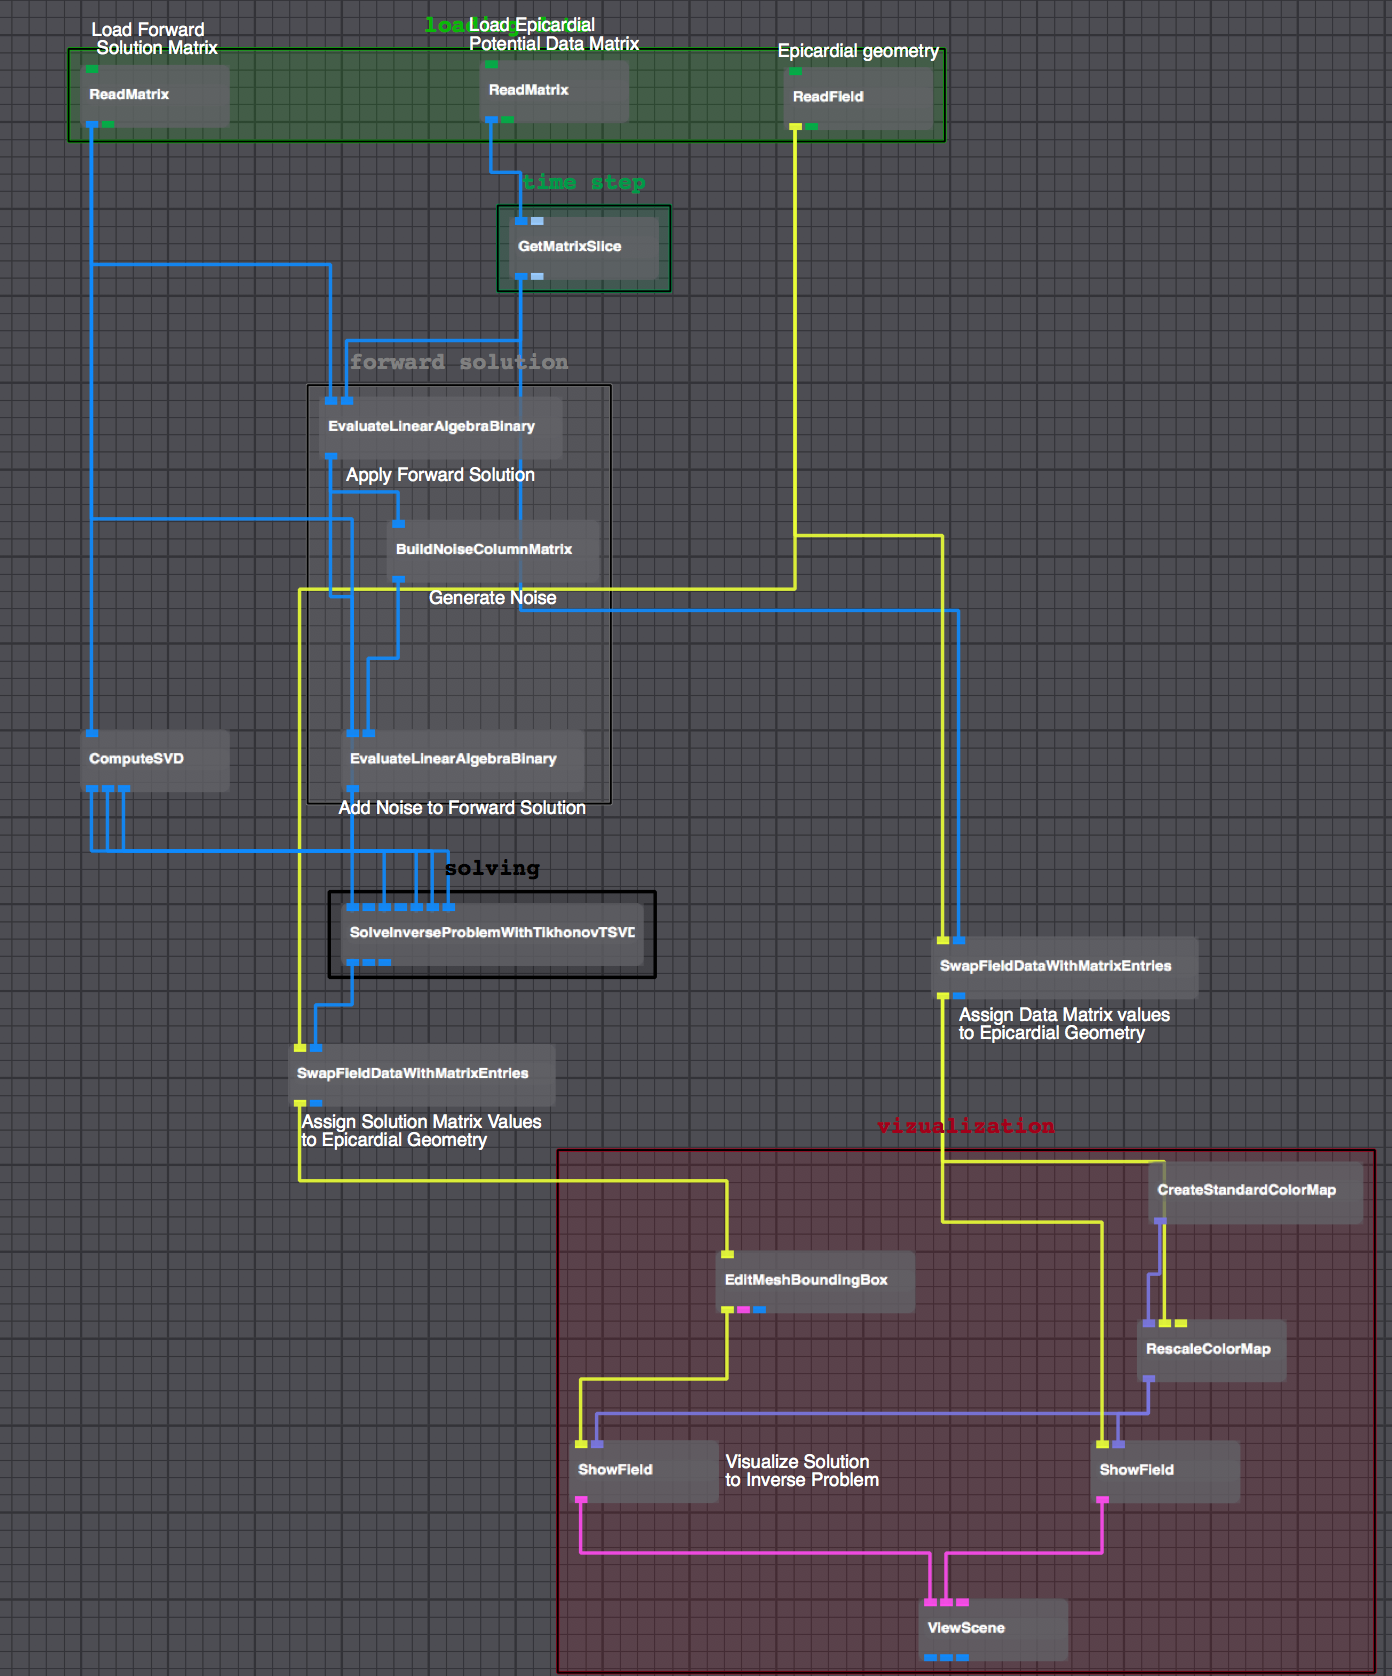
\includegraphics[width=0.9\textwidth]{ECGToolkitGuide_figures/TSVDNetwork.png}
        \caption{The SCIRun network for the TSVD inverse solution example.}
        \label{fig:TSVDNetworkExample}
        \end{center}
    \end{figure}



% \subsection{Total Variation}

%     \subsubsection{Options and Modes of Operation}
    
    
   
% \subsection{Method of Fundamental Solutions}

%     \subsubsection{Options and Modes of Operation}
    
   
\subsection{Isotropy Method}
    
    The Isotropy Method is an approach that considers temporal correlations to imrove the conditioning of the inverse taken. 
    In SCIRun we have implemented this approach with a combination of modules and \href{http://scirundocwiki.sci.utah.edu/SCIRunDocs/index.php/CIBC:Documentation:SCIRun:Reference:BioPSE:SolveInverseProblemWithTikhonov}{{\tt SolveInverseProblemWithTikhonov}}.
    Our implementation of the Isotropy Method can be found in the example network ``potential-based-inverse/greensite-inverse-IsotropyMethod.srn5'', shown in \autoref{fig:IsotropyMethod}.
    
    The network is composed of the standard sections of a simulation network to loading data, visualizing and synthesizing the ECG measurements. 
    The specific blocks that correspond to the Isotropy Method are the ``Temporal Decomposition'', ``solving'' and ``Temporal Reconstruction''. Here we describe this blocks in more detail:
    \begin{enumerate}
        \item The {\bf temporal decomposition} block computes the singular value decomposition of the input data, truncates the right singular vectors (corresponding to time) and projects the input data into this lower dimensional space.
        \item The {\bf solving } block consists on a Tikhonov module that solves the inverse problem for the input data projected onto the low dimensional temporal space.
        \item The {\bf temporal reconstruction} block, uses the truncated right singular vectors from (1) to reconstruct the full temporal behavior of the inverse solutions obtained in the Tikhonov solver.
    \end{enumerate}

    \subsubsection{Options and Modes of Operation}
    
    As implemented, the Isotropy Method does not have many options for operation. The most important parameter that needs to be determined by the user is the truncation point of the right singular vectors, which can be accessed in the ``SelectSubMatrix'' module within the ``temporal decomposition'' block. 
    The GUI for this module, shown in \autoref{fig:IsotropyMethod_gui}, allows to select a submatrix from an input matrix. In the case of the isotropy method, the users are only interested in the ``end'' parameter from the column range selector (lower right entry) since it determined where to truncate the right singular vectors.
    
    This implementation of the Isotropy Method has extra parameters that determine the operation of the Tikhonov inverse. These parameters are specific to the \href{http://scirundocwiki.sci.utah.edu/SCIRunDocs/index.php/CIBC:Documentation:SCIRun:Reference:BioPSE:SolveInverseProblemWithTikhonov}{{\tt SolveInverseProblemWithTikhonov}} module and we refer the user to \autoref{sec:inverse:tikhonov} for more details.
    
%    \begin{figure}
%        \begin{center}
%        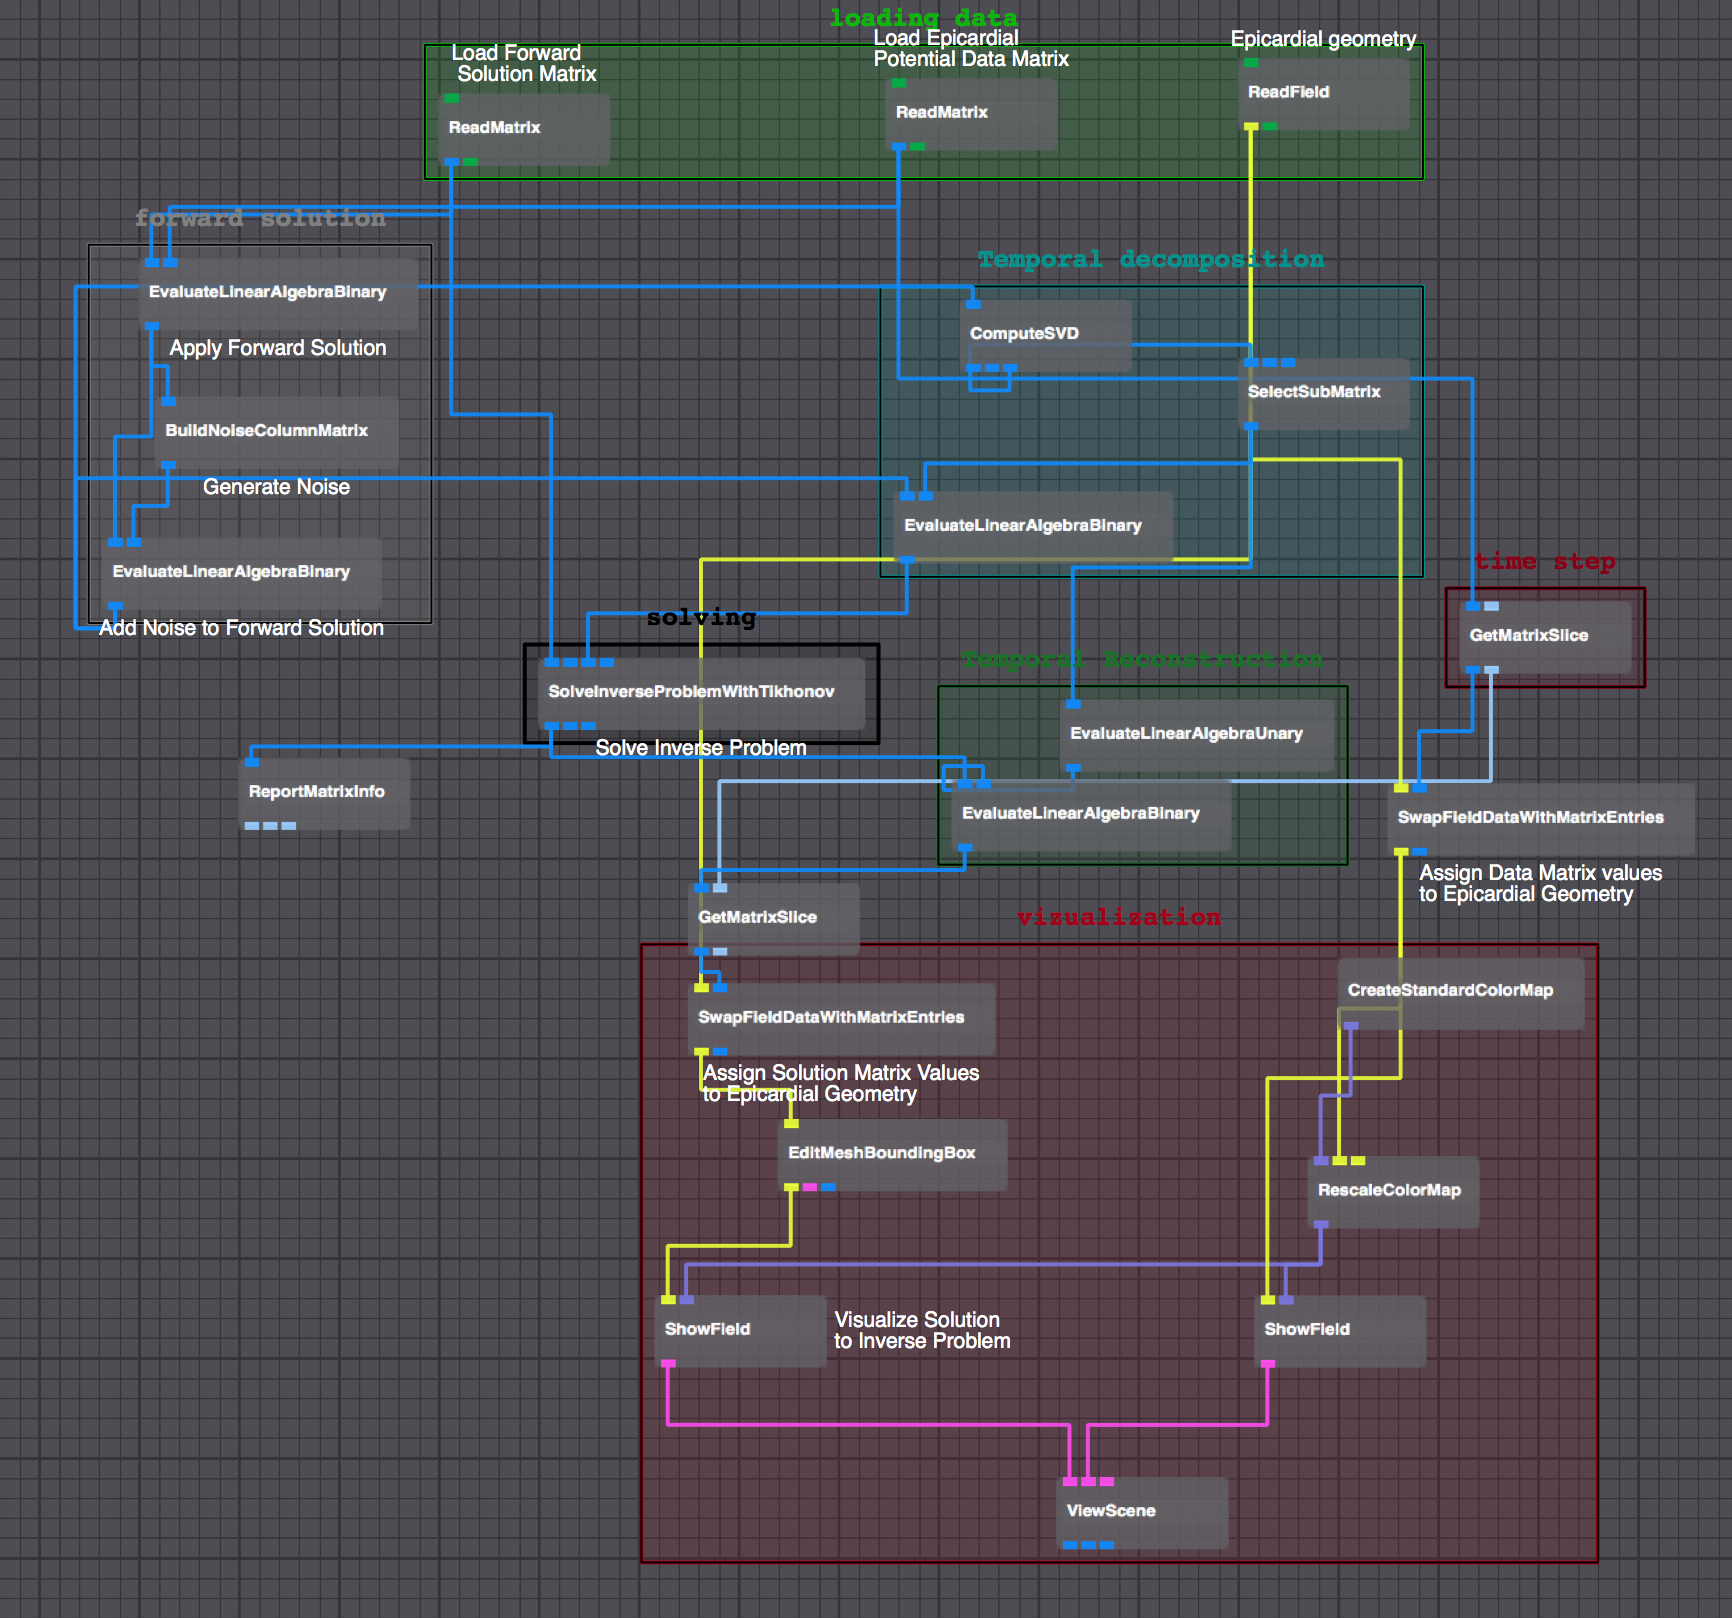
\includegraphics[width=0.9\textwidth]{ECGToolkitGuide_figures/IsotropyMethod_networkExample.png}
%        \caption{The SCIRun network for the Isotropy Method inverse solution example.}
%        \label{fig:IsotropyMethod}
%        \end{center}
%    \end{figure}
    
   
% \subsection{Spline-Based Inverse Method}

%     The spline-based inverse method is another approach that takes into account the temporal characteristics of the signal. In this particular case, it projects the input data onto a 1D manifold characterized with a spline \cite{}.
%     The current implementation of this method uses the MATLAB-python interface capabilities as well as the implemented inverse methods.
%     Similarly to the Isotropy Method, the spline-based inverse is composed of three main blocks ``temporal decomposition'', ``inverse solving'' and ``temporal recontruction''. 
%     The main difference concerns the temporal decomposition and reconstruction steps, which now are non-linear and involve the estimation fo a 1D manifold.
%     In the following, we will describe these three blocks:
    
%     \noindent{\bf Manifold Estimation:}
    
%     \begin{verbatim}
%     %		This code implements the inverse solutions pipeline presented in
%     %		the paper:
%     %	        Erem, Coll-font, Martinez Orellana - 2013 - 
%     %	        Using Transmural Regularization and Dynamic Modeling 
%     %	        for Non-Invasive Cardiac Potential Imaging of 
%     %	        Endocardial Pacing Sites with Imprecise Thoracic Geometry.
%     %
%     %		Inputs
%     %				  i1 - <N,T>double - measured potentials on the torso.
%     %				  i2 - <N,M>double - forward matrix.
%     %				  i3 - <L,M>double - regularization matrix.
%     %				  i4 - <3,1>int - regularization constant params.
%     %				                  i4(1) - log10 min lambda.
%     %				                  i4(2) - log10 max lambda
%     %				                  i4(3) - num lambda.
%     %		Outputs
%     %				  o1 - <M,T>double - estimated heart potentials.
%     \end{verbatim}


%     \noindent{\bf Inverse Solution:}
%     \begin{verbatim}
    
%     \end{verbatim}

%     \begin{figure}
%         \begin{center}
%         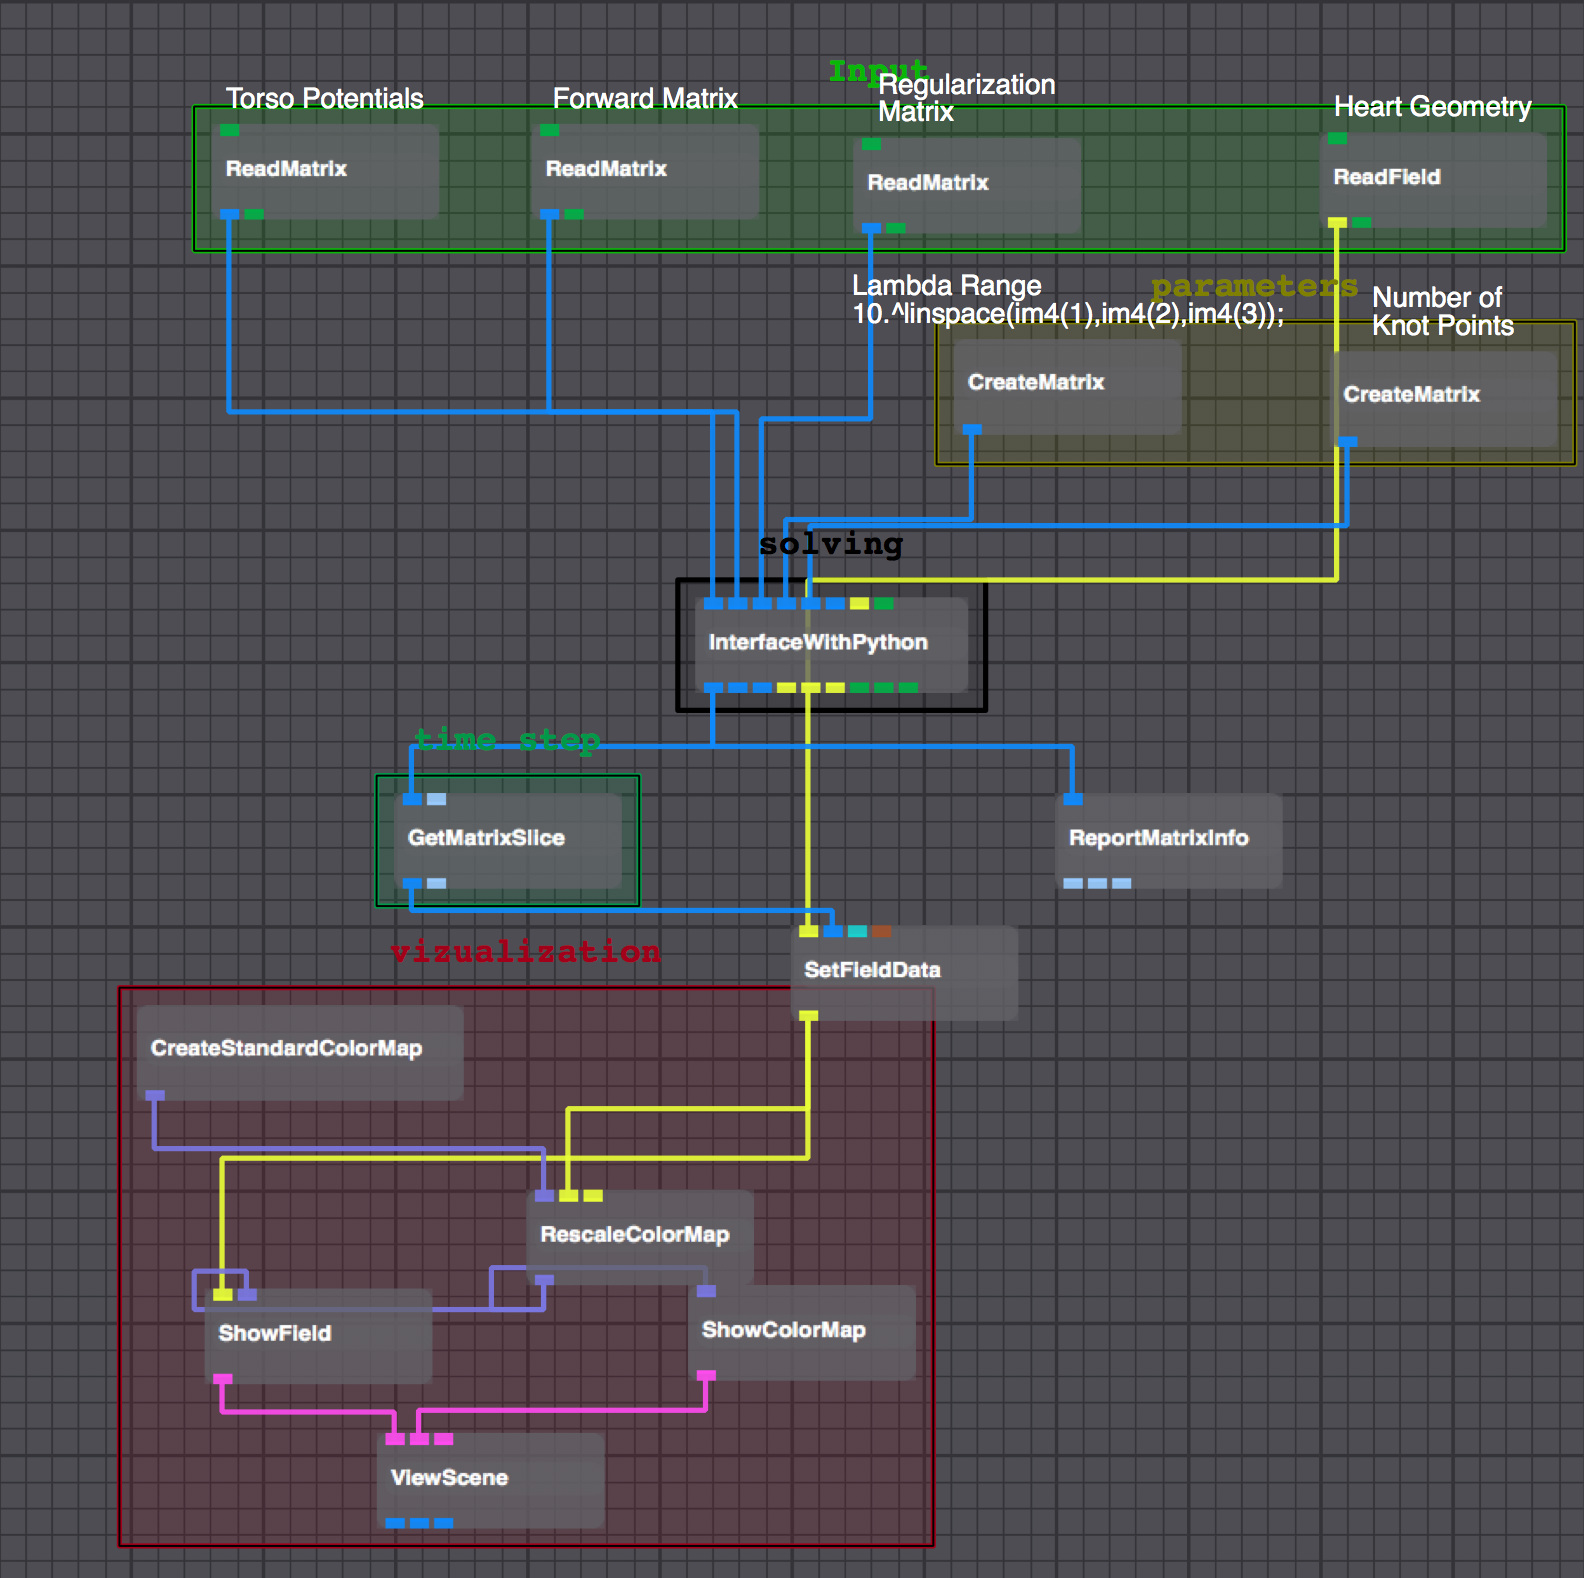
\includegraphics[width=0.9\textwidth]{ECGToolkitGuide_figures/splineInverse_Network.png}
%         \caption{The SCIRun network for the Spline-Based Method inverse solution example.}
%         \label{fig:splineInverse}
%         \end{center}
%     \end{figure}
    
    

% \subsection{Non-Decreasing Inverse Method}

%     The Non-Decreasing Inverse Method estimates the transmembrane potentials by solving a constrained Tikhonov problem.
%     Thus the function to be optimized over is a standard Tikhonov problem but restricts the solutions to always be non-decreasing.
%     Thus, the problem to be solved is:
%     \begin{equation}\begin{split}
%     		\min_{x(t), t=1\dots T} &\|y(t) - Ax(t)\|_2^2 + \lambda*\|Rx(t)\|_2^2 \\
%     		&s.t.\\
%       		&\hspace{2cm}x(1) >= minB\\
%          	&\hspace{2cm}x(t+1) >= x(t), \hspace{.2cm}t=1\dots T-1\\
%          	&\hspace{2cm}x(T) <= maxB
%     \end{split}
%     \end{equation}
%     Where $minB$ and $maxB$ are the minimum and maximum bounds for the TMP.
%     For memory efficiency, this problem is implemented with an ADMM solver.
    
%     This model assumes that the electrical sources of the heart model the transmembrane potentials on each node of the geometry. The inputs and ouputs of the MATLAB implementation can be seen here:
%     \begin{verbatim}
%     %% MESSNARZ INVERSE SCRIPT FOR SCIRUN
%     %
%     %           (...)
%     %			INPUT:
%     % 					- A - <N M>double - forward operator of the linear system.
%     % 					- R - <H,M>double - regularization matrix.
%     % 					- ECG - <N,T>double - Body surface measurements.
%     % 					- lambda - double - regularization term.
%     % 					- initialx - <M,T>double - initial guess for the TMP
%     % 					solution.
%     % 					- rho - double - augmented term weight.
%     % 					- min_r - double - stopping criteria for the primal
%     % 					residual.
%     % 					- min_s - double - stopping criteria for the dual residual.
%     %					- margin - <2,1>double - minimum and maximum bounds for
%     %					the transmembrane potentials.
%     % 					- verbose - boolean - print ADMM iteratinons information.
%     %
%     %			OUTPUT:
%     % 					- xk - <M,T>double - estimated TMP.
%     % 					- zk - <M,T+1>double - estimated slack variable.
%     %           (...)
%     %
%     \end{verbatim}
%     \noindent{\bf Inputs:}
%     \begin{enumerate}
%         \item Forward Matrix ($A\in\Re^{N,M}$)
%         \item Regularization matrix ($R\in\Re^{F,N}$)
%         \item Measured Potentials ($Y\in\Re^{N,T}$)
%         \item Regularization parameter ($\lambda\in\Re$)
%         \item Initial guess for the transmembrane potentials ($X_0\in\Re^{N,1}$ )
%         \item ADMM parameters: weight of augmented lagrangian, stopping paramter for primal and dual objectives ($\rho, min_r, min_s \in\Re^{+}$)
%         \item Lower and upper bounds (margin) of the transmembrane potentials ($marg\in\Re^2$)
%     \end{enumerate}
    
%     \noindent{\bf Outputs:}
%     \begin{enumerate}
%         \item Heart potentials ($xk\in\Re^{M,T}$ )
%     \end{enumerate}
    
%     The resulting potentials have sharp increases of potentials similar to the typically observed in TMPs for most of the nodes on the heart geometry.
%     In general, the final solution is insensitive to the initial guess but it will affect the time of convergence.
%     The script is set up such that the initial guess for the first lambda is a simple ramp, after each initial guess is the final result of the previous lambda. 
%     The decision of the correct lambda is done automatically using an L-corner detection.
%     This algorithm is implemented as the SCIRUN network shown in \autoref{fig:nonDecreasingNetwork}
    
%     NOTE: This code requires the software package reguTools (http://www.imm.dtu.dk/~pcha/Regutools/) to be incorporated in the default path from MATLAB.

%     \subsubsection{Options and Modes of Operation}
%     \begin{figure}
%         \begin{center}
%         \includegraphics[width=0.9\textwidth]{ECGToolkitGuide_figures/nonDecreasingNetwork.png}
%         \caption{The SCIRun network for the Non-Decreasing Inverse Method inverse solution example.}
%         \label{fig:nonDecreasingNetwork}
%         \end{center}
%     \end{figure}


   
\subsection{Activation-Based Method}
    
    The activation-based inverse method solves the inverse problem in electrocardiography through the estimation of the activation times (\emph{i.e.} the depolarization times) on the heart.
    This inverse method assumes that the sources on the heart are modeled with a potentials over time at each node are parameterized  by the time of activation.
    This assumption allows the inverse method to resolve the inverse problem by estimating the activation times at every node on the heart geometry.
    
    The inverse problem being solved is thus a non-linear optimization problem for which there is no closed-form solution. 
    The implementation of the activation-based inverse in SCIRun is done with a Gauss-Newton iterative method that solves:
    \begin{center}
        \begin{eqnarray}
            min_{X} \|Y - A \Phi(\tau, \omega) \|^{2}_{2} + \lambda \| R\Phi(\tau, \omega) \|^{2}_{2},
        \label{eq:inverseSec_actBasedObj}
        \end{eqnarray}
    \end{center}
    where $\Phi(\cdot)$ is the pre-defined temporal waveform at each node and is paramaterized by $\tau$ and $\omega$, which correspond to the time of activation and the slope of the depolarixzation wave respectively.
    $Y$ are the measured body surface potentials, $A$ the forward matrix and $R$ the regularization matrix.
    
    The inputs and outputs of this inverse method can be observed in the ``InterfaceWithPython'' module in the network example shown in \autoref{fig:activationBasedNetwork} and in the header of the MATLAB implementation:
    \begin{verbatim}
        function tau = ActGaussNewton(A,Y,L,tauinit,lambda,w,minstep)
        % Implements the Gauss-Newton algorithm for solving the activation-based
        % inverse problem of electrocardiography.
        % => minimizes the objective function ||Y-A*X||^2+lambda*||L*X||^2 where
        % X is parameterized by the C^1 polynomial approximation to a step function
        % as explained in "The Depolarization Sequence of the Human Heart Surface
        % Computed from Measured Body Surface Potentials" by Geertjan Huiskamp and
        % Adriaan van Oosterom.
        %
        % Input Variables:
        % A: Forward matrix
        % Y: Observations (columns index time from 1 to T=size(Y,2))
        % L: Regularization matrix (typically a surface Laplacian approximation)
        % lambda: Regularization parameter
        % w: Width parameter in step function approximation
        % tauinit: Initial phase shifts for starting the algorithm
        %
        % Output Variables:
        % tau: Solution phase shifts of the step functions
    \end{verbatim}
    
    \noindent{\bf Inputs:}
    \begin{enumerate}
        \item Forward Matrix ($A\in\Re^{N,M}$)
        \item Measured Potentials ($Y\in\Re^{N,T}$)
        \item Regularization matrix ($R\in\Re^{F,N}$)
        \item Initial guess for the activation times ($\tau\in\Re^{N,1}$ )
        \item Regularization parameter ($\lambda\in\Re$)
        \item Activation waveform transition width ($\omega\in\Re^{+}$)
        \item Convergence parameter ($\epsilon\in\Re^{+}$)
    \end{enumerate}
    The initial guess is the set of activation times from which the Gauss-Newton algorithm starts pursuing a more suitable inverse solution. 
    The transition width controls the number of time samples (not necessarily integer) taken by each source to transition from inactivated to activated in this method. 
    The convergence parameter is the minimum norm of the step taken by the iterations within the Gauss-Newton algorithm before the method is deemed to have converged to a suitable solution. 
    
    \noindent{\bf Outputs:}
    \begin{enumerate}
        \item Activation times ($\tau\in\Re^{M,1}$ )
    \end{enumerate}
    The only output of the method is the inverse solution in the form of an array of activation times.
    
%    \begin{figure}
%        \begin{center}
%        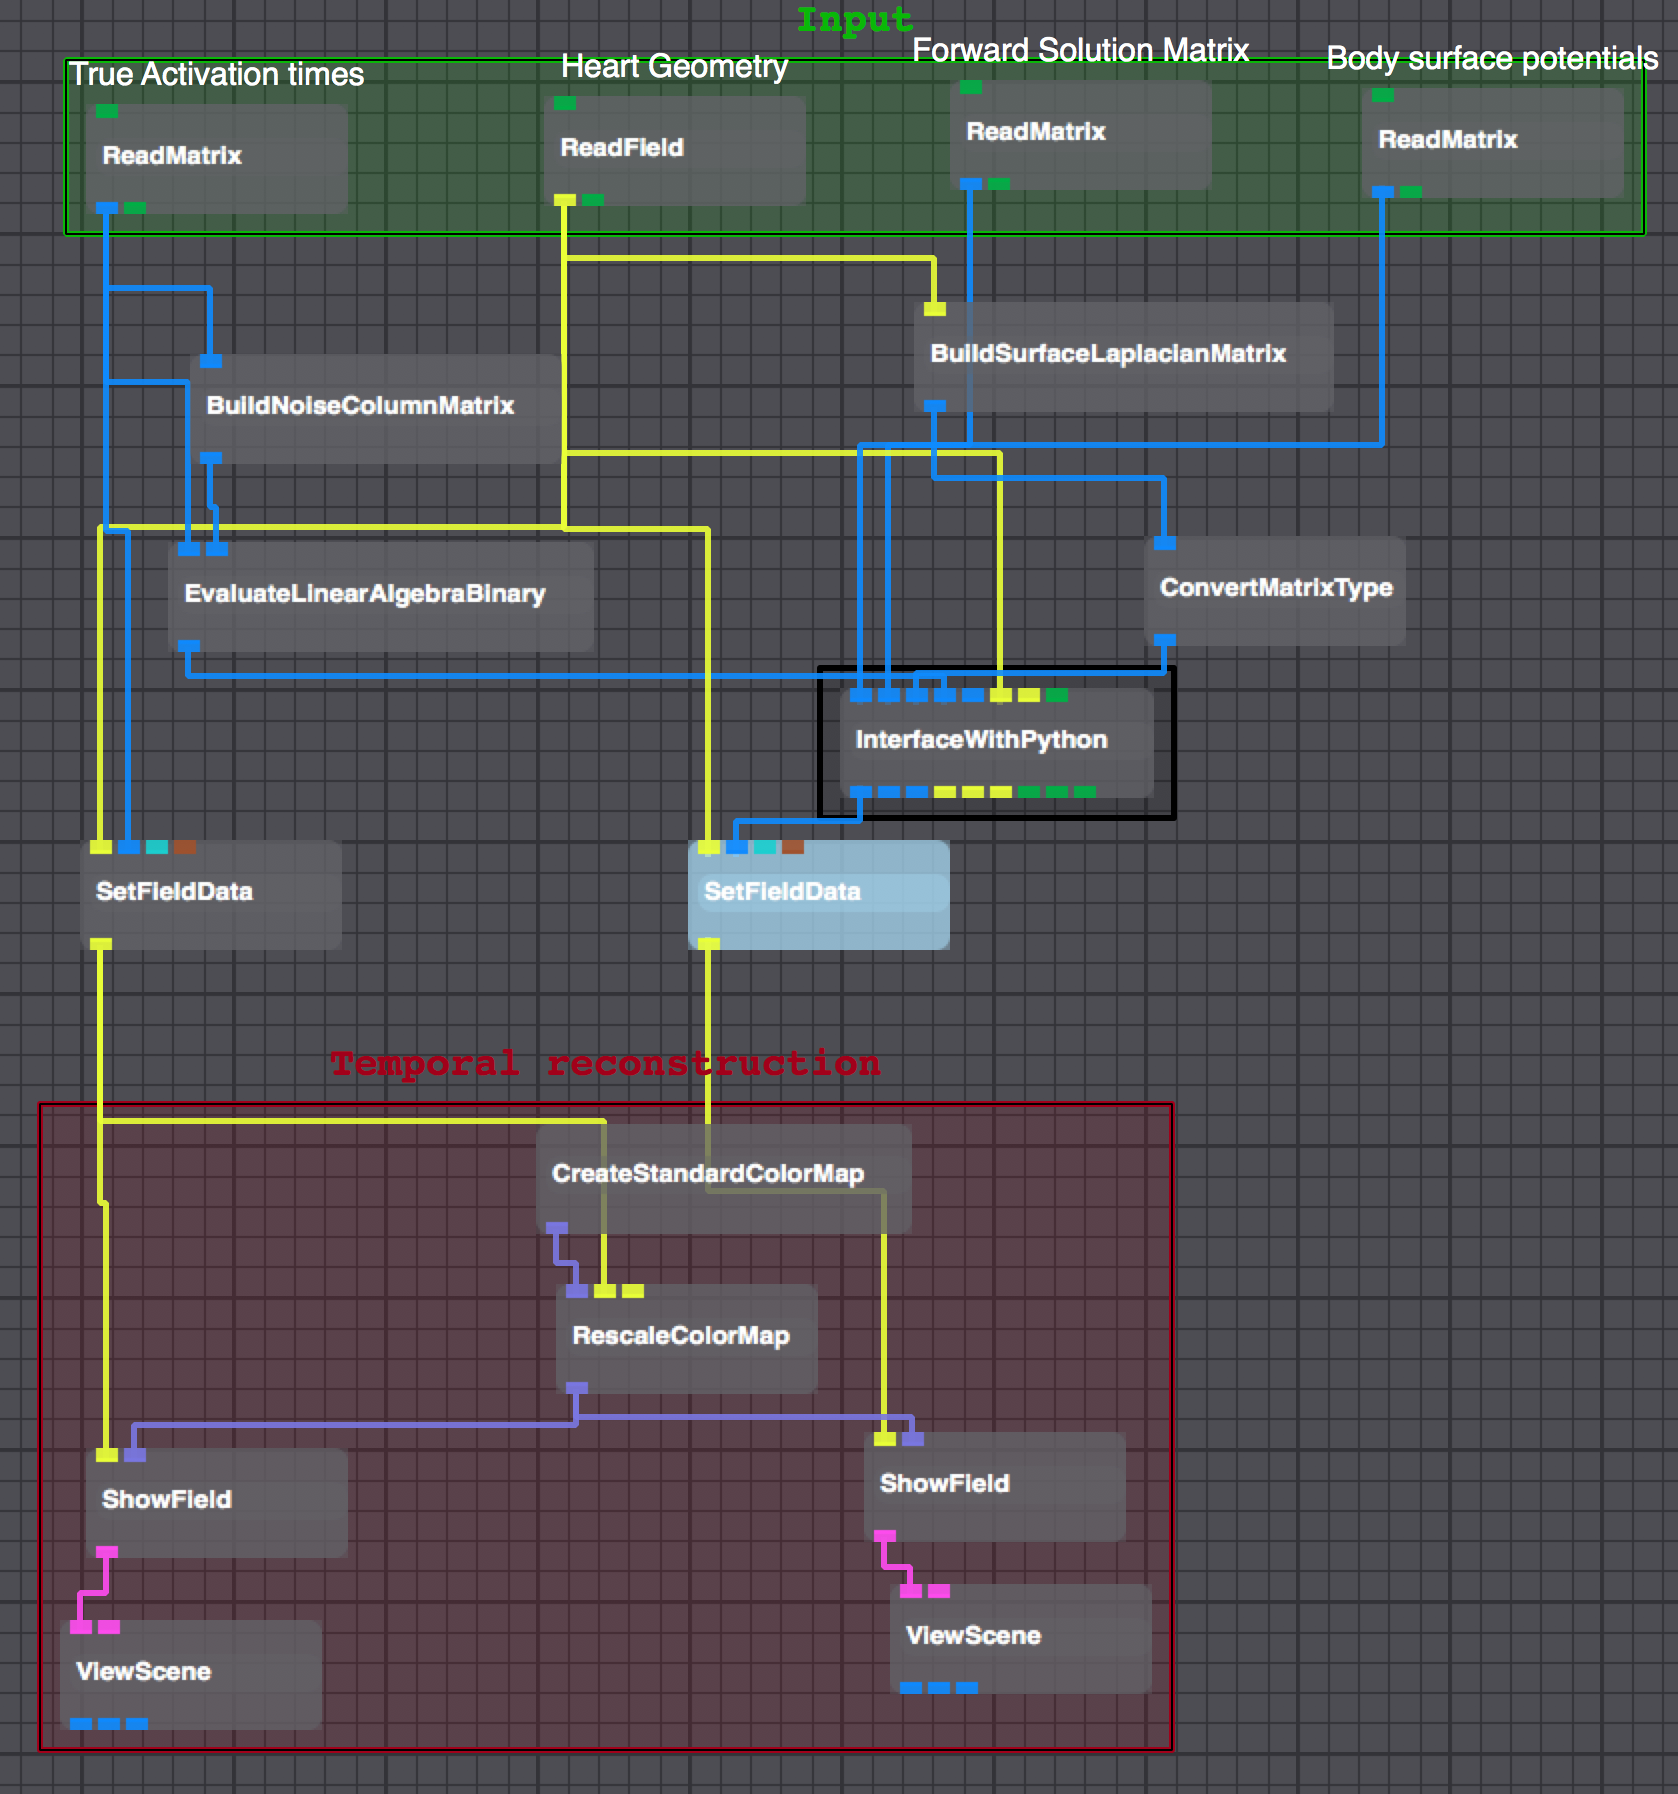
\includegraphics[width=0.9\textwidth]{ECGToolkitGuide_figures/activationBasedNetwork.png}
%        \caption{The SCIRun network for the Activation-Based Method inverse solution example.}
%        \label{fig:activationBasedNetwork}
%        \end{center}
%    \end{figure}


% \subsection{Wavefront-Based Potential Reconstruction (WBPR)}

%     The Wavefront-Based Potential Reconstruction (WBPR) method imposes prior knowledge about the spatial patterns of electric potentials on the heart during the QRS complex to reconstruct an inverse solution. 
%     This inverse method assumes a source model characterizing the extracellular potentials on the heart surface and introduces a regularization term that imposes them to be similar to a pre-specified shape.
    
%     The inputs and outputs of this inverse method can be observed in the ``InterfaceWithPython'' module in the network example shown in \autoref{fig:WBPRNetwork} and in the header of the MATLAB implementation:
%     \begin{verbatim}
%     function [x_WBPR_forward,x_WBPR_backward] = WBPR(A,y,heart,first_act,last_act)
%     % Function to calculate the WBPR solutions
%     % Inputs:
%     %   A: forward matrix
%     %   y: torso data
%     %   heart: heart geometry
%     %   first_act: first activated node
%     %   last_act: last activated node
%     %
%     % Outputs:
%     %   x_WBPR_forward: inverse solution using forward WBPR
%     %   x_WBPR_backward: inverse solution using backward WBPR
%     \end{verbatim}

%     \noindent{\bf Inputs:}
%     \begin{enumerate}
%         \item Forward Matrix ($A\in\Re^{N,M}$)
%         \item Measured Potentials ($Y\in\Re^{N,T}$)
%         \item Heart geometry (struct containing nodes and triangles)
%         \item First and last nodes to activate ()
%     \end{enumerate}
   
%     \noindent{\bf Outputs:}
%     \begin{enumerate}
%         \item forward WBPR solution ($X_f\in\Re^{M,T}$ )
%         \item backward WBPR solution ($X_b\in\Re^{M,T}$ )
%     \end{enumerate}
%     As output, WBPR produces two inverse solutions. The procedure by which the inverse solutions are obtained may be run both forward and backward in time. Therefore, the ``forward WBPR'' solution is that obtained by applying the method starting from the earliest sample time and ending at the latest. On the other hand, the ``backward WBPR'' solution is obtained by starting from the latest sample time and traversing the samples in reverse until ending at the earliest.

%     NOTE: This code requires the software package reguTools (http://www.imm.dtu.dk/~pcha/Regutools/) to be incorporated in the default path from MATLAB.

%     \begin{figure}
%         \begin{center}
%         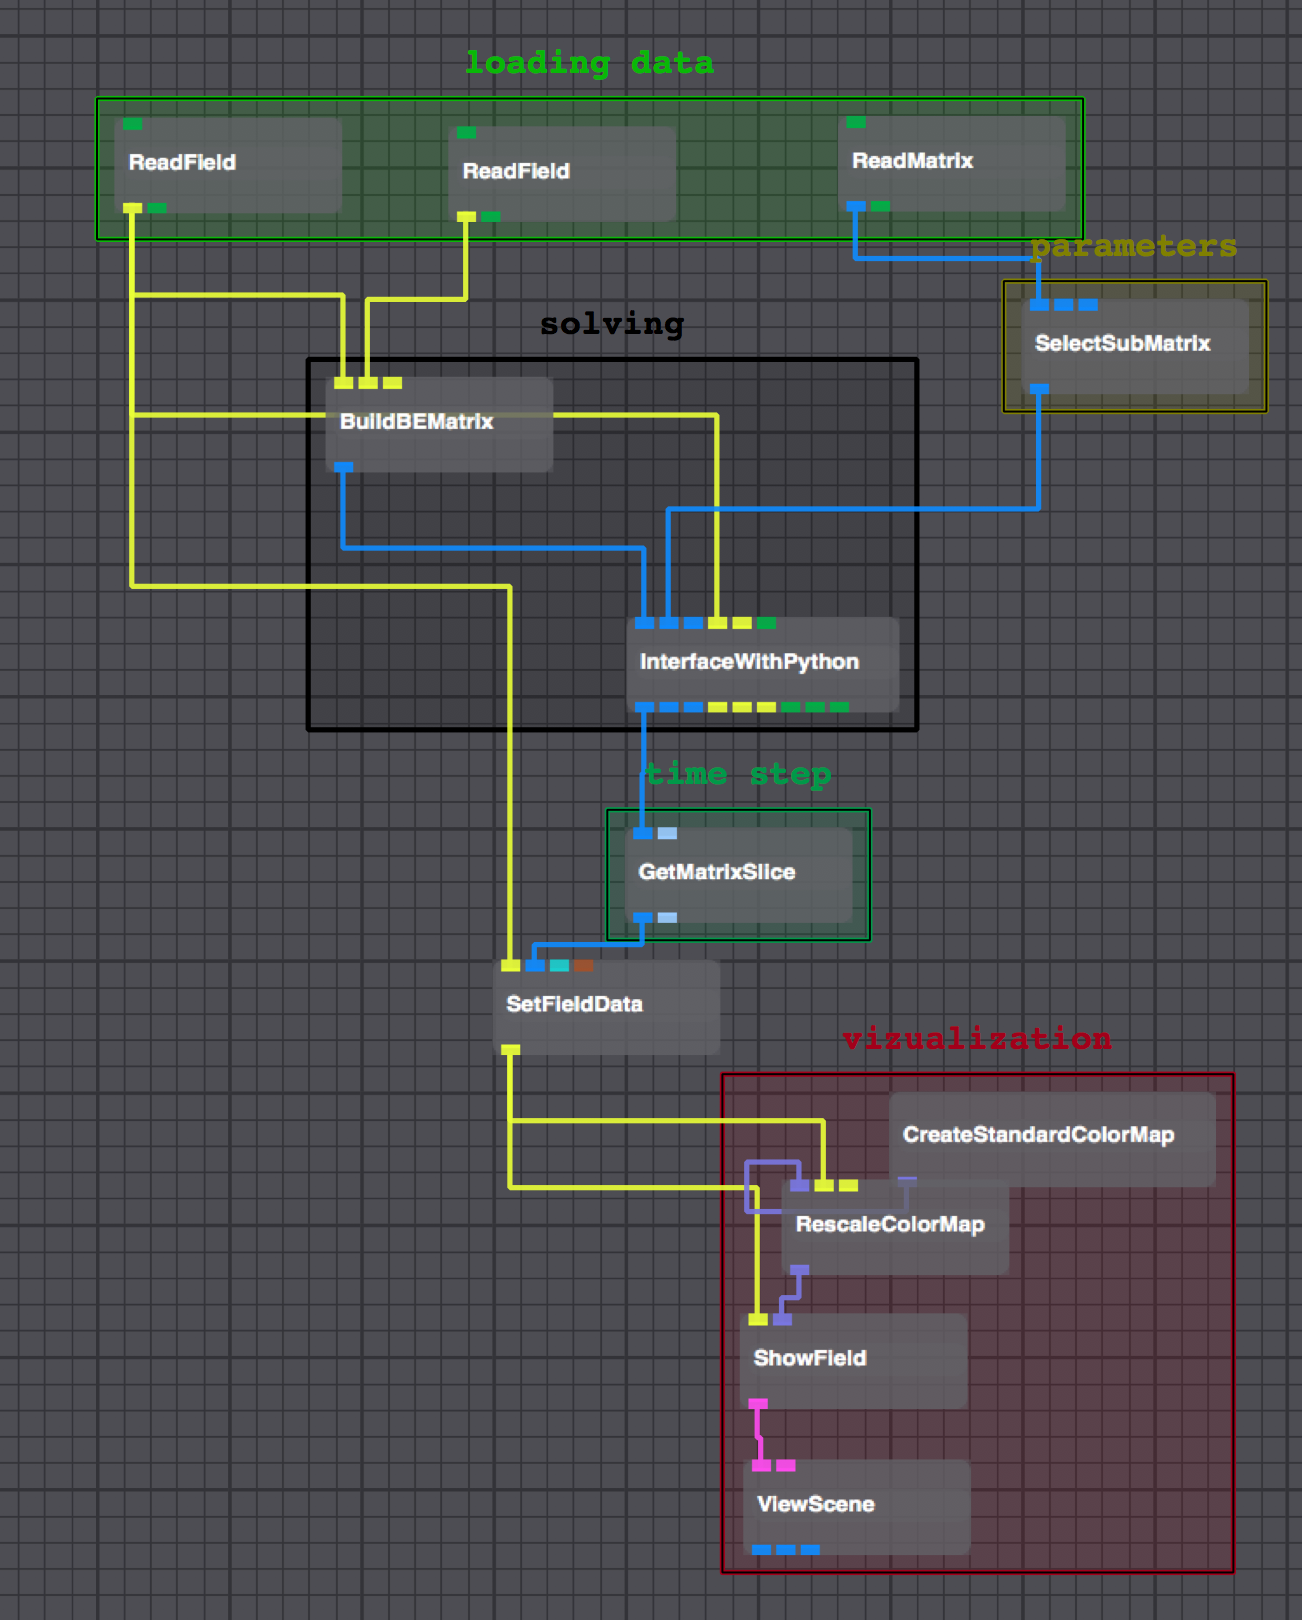
\includegraphics[width=0.9\textwidth]{ECGToolkitGuide_figures/WBPRNetwork.png}
%         \caption{The SCIRun network for the WBPR Method inverse solution example.}
%         \label{fig:WBPRNetwork}
%         \end{center}
%     \end{figure}

